% =====================================================================
% SICA: short course project report (maximum four pages).
% All numbers are taken unchanged from the stored results in
% ../results/tables; nothing here was re-run or re-tuned.
% Build: pdflatex report && bibtex report && pdflatex report && pdflatex report
% =====================================================================
\documentclass[conference]{IEEEtran}
\IEEEoverridecommandlockouts
\usepackage[T1]{fontenc}
\usepackage{cite}
\usepackage{amsmath,amssymb}
\usepackage{graphicx}
\usepackage{booktabs}
\usepackage{array}
\usepackage{xcolor}
\usepackage{tikz}
\usetikzlibrary{positioning,fit,backgrounds,calc,arrows.meta}
\usepackage[hidelinks]{hyperref}
\usepackage{microtype}

\definecolor{rblue}{RGB}{31,78,121}
\definecolor{rred}{RGB}{192,80,77}

\begin{document}

\title{Detecting Mid-Session HTTP Session Hijacking from Server Access Logs Using Client-Binding Forks\\[0.6ex]
{\large Computer Security Course Project Report}}

\author{%
\IEEEauthorblockN{%
\begin{tabular}{c@{\hspace{2.2em}}c@{\hspace{2.2em}}c}
Shadhin Nandi & Md. Nurul Alam Siddiqei Ador & Mueen Ishraq Ananta\\[-0.2ex]
{\normalsize\normalfont ID: 0112230604} & {\normalsize\normalfont ID: 0112230170} & {\normalsize\normalfont ID: 0112230155}
\end{tabular}}
\IEEEauthorblockA{Department of Computer Science and Engineering (CSE), United International University (UIU), Dhaka, Bangladesh\\[0.8ex]
\textit{Supervisor:} Dr. Muhammad Nomani Kabir, Professor, Department of CSE, United International University}}

\maketitle

\begin{abstract}
After login, a web application recognises a user only by a session identifier,
so an attacker who steals it can act inside the session without any failed
login. Binding the session to the client's IP address is a common defence, but
honest users also change networks, which causes false alarms. In this project we
built SICA (Session Integrity and Continuity Analysis), a detector that uses
only web server access logs. SICA describes each request by a client binding
(IP address, /24 and /16 network, browser, operating system and device) and
checks for agent changes, graded network changes and binding forks, where an
earlier binding returns after a different one, as happens when a victim and an
attacker share a session. The checks form a risk score that is compared with a
threshold calibrated on attack-free sessions. On two public access-log datasets
with injected hijacks, SICA reached ROC AUC 0.884 and 0.851 with false-positive
rates below 1\% and precision above 0.9. Recall was low (0.358 and 0.229):
attackers who copy the victim's binding, and most silent takeovers, are missed.
\end{abstract}

\begin{IEEEkeywords}
session hijacking, web access logs, client binding, anomaly detection
\end{IEEEkeywords}

% =====================================================================
\section{Introduction}
% =====================================================================

HTTP is stateless, so a web application keeps a user logged in by giving the
browser a session identifier after authentication, normally in a
cookie~\cite{rfc6265}. From then on the identifier is the only proof of identity
the server checks. Whoever presents it is treated as the user. Attackers can
obtain it through cross-site scripting, network interception, malware or leaked
logs, and measurements on popular services have shown that stolen session
cookies can expose private user data in
practice~\cite{sivakorn2016cookie,calzavara2017surviving}.

Detecting a stolen session after login is difficult. The attacker never
authenticates, so there is no wrong password to notice, and each request carries
a valid identifier with content that can look exactly like the victim's. The
only evidence lies in the context: which network the requests come from, which
client software sends them, and how this changes during the session.

The usual server-side rule is to bind the session to the client's IP address and
end it when the address changes. The main problem is that legitimate users also
change addresses. Dynamic addresses are renumbered~\cite{padmanabhan2016dynamic},
and a phone may move from Wi-Fi to a mobile network in the middle of a session.
An IP pin treats each of these as an attack, and its false-alarm rate is simply
the rate at which honest users move, which the operator cannot tune. Since real
hijacks are rare compared with normal sessions, even a few percent of false
alarms means that most alerts are false~\cite{axelsson2000baserate}. A richer
client binding helps here. A new host in the same /24 network is weak evidence,
while a jump to a different network, or a switch to a different browser or
operating system, is much stronger.

Previous work has approached session theft from several directions. Some
defences make a stolen token useless, for example by replacing the static cookie
with per-request tokens, which needs support in both browser and
server~\cite{dacosta2012onetime}. A survey of web session security notes that
most proposed defences work in the browser, in the protocol or in the
application code~\cite{calzavara2017surviving}. SHPF binds the session to a
browser fingerprint collected with JavaScript and ends the session when the
fingerprint changes~\cite{unger2013shpf}. Risk-based authentication compares the
IP address and User-Agent of a login with the user's login
history~\cite{freeman2016whoareyou}. Log-based detectors learn models of web
request parameters~\cite{kruegel2003anomaly} or of system log sequences with deep
learning~\cite{du2017deeplog}. These studies show that client context is a
useful security signal, but they need client changes or JavaScript, work only at
login time with per-user history, or depend on trained models of request
content.

Our project looks at a narrower, practical question: \emph{can a server detect
observable mid-session hijacking using only the access logs it already writes,
while keeping the false-alarm rate controlled and each alert easy to explain?}
Our answer is SICA. It is based on one observation about the shape of binding
changes. A user who moves from binding $A$ to binding $B$ leaves $A$ behind
($A\,A\,A\,B\,B\,B$). When an attacker uses a stolen session while the victim is
still browsing, the two clients alternate and the earlier binding comes back
($A\,A\,B\,A\,B$). We call this return a \emph{binding fork}.

In summary, we (i) built a client binding from access-log fields only, (ii)
defined three simple checks, including the binding fork, (iii) derived the
weights and a single alert threshold from attack-free sessions, without attack
labels or machine learning, and (iv) evaluated SICA on two public access-log
datasets and compared it with IP pinning.

% =====================================================================
\section{Methodology}
% =====================================================================

\subsection{Problem Definition}

A web server logs each request with the client IP address, time, requested path,
status code, response size, referrer and User-Agent string. A session is the
ordered list of requests that present the same session identifier. For every
session, SICA must decide ALLOW or ALERT from the log alone, while keeping the
share of benign sessions that alert close to a budget chosen in advance. We
consider two kinds of hijack: a \emph{silent takeover}, where the victim stops
sending requests after the theft, and a \emph{concurrent hijack}, where the
victim and the attacker both keep using the session.

\subsection{Client Binding}

Each request is mapped to a client binding with seven fields:
\begin{center}
IP address \;|\; /24 \;|\; /16 \;|\; browser \;|\; version \;|\; OS \;|\; device
\end{center}
The first three fields form the \emph{network part}, and the last four, parsed
from the User-Agent string, form the \emph{agent part}. Together they describe
the client at different levels of detail. A new host in the same /24 is typical
of an address renewal. A new /24 inside the same /16 often means another access
network of the same provider. A new /16 usually means the client has left the
network where the session started. On the agent side, a version change can
follow a browser update, but a real client does not switch to a different
browser, operating system or device class in the middle of a session.

For each live session, SICA keeps a \emph{reference binding} and a list of the
last four distinct bindings. When a client makes a one-way move to a new
binding, the reference moves with it, so a user who settles on a new network is
counted only once. When an earlier binding returns, the reference is left
unchanged, because with two clients alternating there is no way to tell which
one is the owner.

\subsection{The Three Checks}

\textbf{V1: Agent mutation.} V1 compares the agent part of the request with the
reference. It is 1.00 if the browser family, operating system or device class
changed, and 0.35 if only the major browser version changed. A version change
receives a smaller value because it can come from a normal update.

\textbf{V2: Network-scope discontinuity.} V2 measures how far the client moved
in the network hierarchy relative to the reference:
\begin{center}
\small
\begin{tabular}{@{}lc@{}}
\toprule
Change relative to the reference & V2 \\
\midrule
new /16 network & 1.00 \\
new /24 inside the same /16 & 0.45 \\
new host inside the same /24 & 0.15 \\
\bottomrule
\end{tabular}
\end{center}
The value is graded instead of a simple ``changed or not changed''. This is the
main difference from an IP pin: a small move inside the same network costs
little, while leaving the /16 network costs the full value.

\textbf{V3: Binding fork.} V3 does not look at the size of a change but at its
shape. It is 1.00 when the binding of the current request differs from the
binding of the previous request but matches a binding that is still in the
list of recent bindings. Consider two sessions:
\begin{center}
\begin{tabular}{@{}l@{\quad}l@{}}
Legitimate move: & \texttt{A A A A B B B B}\\
Concurrent hijack: & \texttt{A A A B A B A}
\end{tabular}
\end{center}
In the first session, $B$ is new, so V3 stays 0. In the second, $A$ returns after
$B$ has appeared. A single client that moves once cannot keep producing this
pattern, while two clients sharing one session cannot avoid it. The fork
therefore suggests that two different clients are using the same session at the
same time. Since the binding includes the full IP address, two hosts that
alternate inside the same /24 are still seen as two bindings.

\subsection{Risk Score}

The three values are combined into a risk score for every request:
\begin{equation}
R = w_1 V_1 + w_2 V_2 + w_3 V_3 .
\end{equation}
The weights are positive and add up to one, so $R$ lies between 0 and 1. They
come from how rare each check is on normal traffic: a check that seldom fires on
benign requests is stronger evidence and receives a larger weight. Concretely,
each weight is proportional to $\ln\bigl(1/(\varepsilon_i+0.01)\bigr)$, where
$\varepsilon_i$ is the average value of check $i$ on attack-free requests. The
session keeps its peak risk $R_{\max}$, the highest request risk seen so far.

\subsection{Calibrated Threshold}

The threshold $\tau$ is selected from benign sessions so that no more than about
1\% of the calibration sessions would trigger an alert. SICA replays the
attack-free calibration sessions, records the peak risk of each one, and picks
the smallest observed peak that keeps at most 1\% of the sessions at or above it.
We scan the observed values instead of taking a plain percentile because many
sessions share exactly the same peak, and a percentile that lands on a tied
value could let too many sessions through. A session is alerted as soon as
$R_{\max}\ge\tau$. There is one threshold per dataset, nothing is learned per
user, and no attack labels are used anywhere.

\subsection{Overall Workflow}

Fig.~\ref{fig:arch} shows the complete pipeline, from the raw access log to the
final decision. Calibration is done once per dataset on attack-free sessions;
after that, the weights and threshold are fixed and every new request is
processed in constant time.

\begin{figure}[t]
\centering
% Figure for report.tex: complete SICA workflow in one column, with its own
% styles so the file is self-contained.
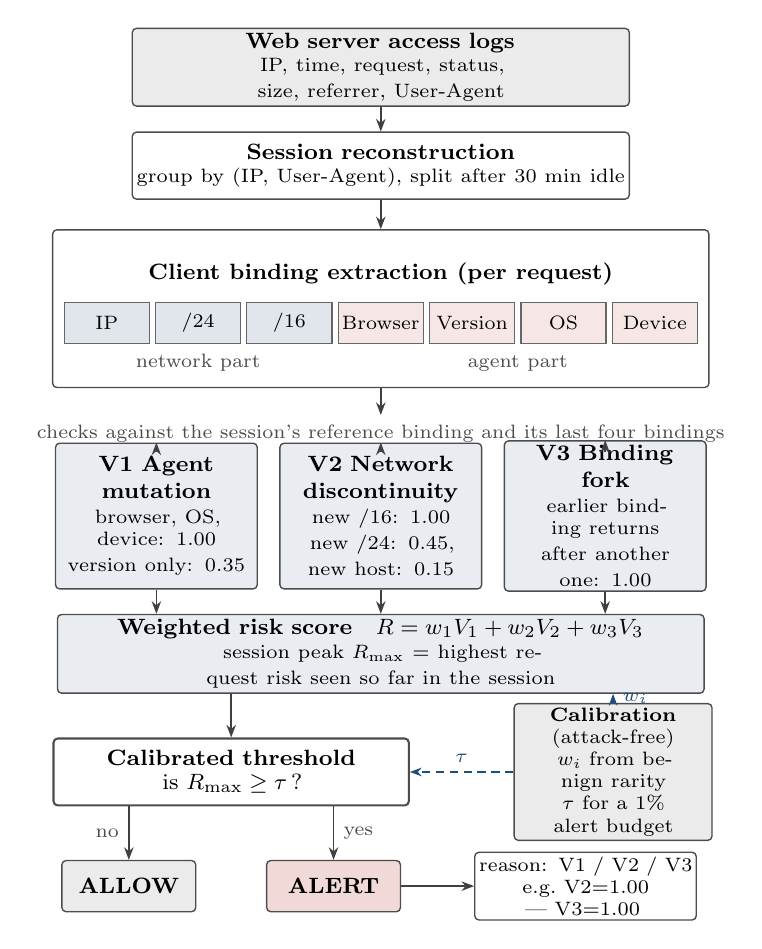
\begin{tikzpicture}[
  x=1mm, y=1mm, font=\footnotesize,
  rbox/.style={draw=black!70, line width=0.5pt, rounded corners=1.5pt, align=center,
               fill=white, inner sep=1.6pt, minimum height=8.5mm},
  rcell/.style={draw=black!60, line width=0.4pt, fill=white, minimum width=10.8mm,
                minimum height=5.2mm, inner sep=0pt, font=\scriptsize},
  rchk/.style={rbox, fill=rblue!10, text width=24.5mm, minimum height=18.5mm},
  rout/.style={rbox, font=\footnotesize\bfseries, minimum width=17mm, minimum height=6.5mm},
  rarr/.style={-{Stealth[length=1.6mm,width=1.2mm]}, line width=0.55pt, draw=black!75},
  rcal/.style={-{Stealth[length=1.5mm,width=1.1mm]}, line width=0.5pt, draw=rblue, densely dashed},
  rsub/.style={font=\scriptsize, text=black!70},
]
  % 1. input
  \node[rbox, fill=black!8, text width=62mm] (log) at (0,3)
    {\textbf{Web server access logs}\\[-0.3ex]
     {\scriptsize IP, time, request, status, size, referrer, User-Agent}};
  % 2. sessions
  \node[rbox, text width=62mm] (sess) at (0,-9.5)
    {\textbf{Session reconstruction}\\[-0.3ex]
     {\scriptsize group by (IP, User-Agent), split after 30 min idle}};
  % 3. binding
  \node[font=\footnotesize\bfseries] (btitle) at (0,-23.2) {Client binding extraction (per request)};
  \foreach \lab [count=\i] in {IP,/24,/16,Browser,Version,OS,Device} {
    \pgfmathsetmacro{\xx}{(\i-4)*11.6}
    \ifnum\i<4 \node[rcell, fill=rblue!14] (c\i) at (\xx,-29.5) {\lab};
    \else \node[rcell, fill=rred!14] (c\i) at (\xx,-29.5) {\lab};\fi
  }
  \node[rsub] at ($(c1.south)!0.5!(c3.south)+(0,-2.4)$) {network part};
  \node[rsub] at ($(c4.south)!0.5!(c7.south)+(0,-2.4)$) {agent part};
  \begin{scope}[on background layer]
    \node[draw=black!70, line width=0.5pt, rounded corners=1.5pt, fill=white,
          fit=(btitle)(c1)(c7), inner xsep=1.4mm, inner ysep=4.2mm, yshift=-1.3mm] (bind) {};
  \end{scope}
  % 4. checks
  \node[rsub, align=center] (chktitle) at (0,-43.5)
    {checks against the session's reference binding and its last four bindings};
  \node[rchk] (v1) at (-28.5,-54)
    {\textbf{V1 Agent}\\\textbf{mutation}\\[0.3ex]
     {\scriptsize browser, OS, device: 1.00\\ version only: 0.35}};
  \node[rchk] (v2) at (0,-54)
    {\textbf{V2 Network}\\\textbf{discontinuity}\\[0.3ex]
     {\scriptsize new /16: 1.00\\ new /24: 0.45,\; new host: 0.15}};
  \node[rchk] (v3) at (28.5,-54)
    {\textbf{V3 Binding}\\\textbf{fork}\\[0.3ex]
     {\scriptsize earlier binding returns\\ after another one: 1.00}};
  % 5. risk and threshold
  \node[rbox, fill=rblue!10, text width=81mm] (risk) at (0,-71.5)
    {\textbf{Weighted risk score}\quad \mbox{$R=w_1V_1+w_2V_2+w_3V_3$}\\[-0.2ex]
     {\scriptsize session peak $R_{\max}$ = highest request risk seen so far in the session}};
  \node[rbox, text width=44mm, line width=0.75pt] (thr) at (-19,-86.5)
    {\textbf{Calibrated threshold}\\[-0.2ex] is \mbox{$R_{\max}\ge\tau$\,?}};
  \node[rbox, fill=black!8, text width=24mm, font=\scriptsize] (cal) at (29.5,-86.5)
    {\textbf{Calibration} (attack-free)\\ $w_i$ from benign rarity\\ $\tau$ for a 1\% alert budget};
  % 6. outputs
  \node[rout, fill=black!8] (allow) at (-32,-101) {ALLOW};
  \node[rout, fill=rred!22] (alert) at (-6,-101) {ALERT};
  \node[rbox, font=\scriptsize, text width=27mm, minimum height=6.5mm] (why) at (26,-101)
    {reason: V1 / V2 / V3\\ e.g.\ V2=1.00 | V3=1.00};
  % arrows
  \draw[rarr] (log) -- (sess);
  \draw[rarr] (sess) -- (bind.north |- sess.south) -- (bind.north);
  \draw[rarr] (bind.south) -- (chktitle.north);
  \foreach \v in {v1,v2,v3} \draw[rarr] (chktitle.south -| \v.north) -- (\v.north);
  \foreach \v in {v1,v2,v3} \draw[rarr] (\v.south) -- (\v.south |- risk.north) ;
  \draw[rarr] (risk.south -| thr.north) -- (thr.north);
  \draw[rarr] (thr.south -| allow.north) -- node[rsub, left] {no} (allow.north);
  \draw[rarr] (thr.south -| alert.north) -- node[rsub, right] {yes} (alert.north);
  \draw[rarr] (alert) -- (why);
  \draw[rcal] (cal.north) -- node[rsub, right, text=rblue] {$w_i$} (cal.north |- risk.south);
  \draw[rcal] (cal.west) -- node[rsub, above, text=rblue] {$\tau$} (thr.east);
\end{tikzpicture}

\caption{SICA architecture. Access-log requests are grouped into sessions and
turned into client bindings. Three checks score each request, their weighted sum
gives the session risk, and a threshold calibrated on attack-free sessions
decides ALLOW or ALERT. Every alert names the checks that caused it.}
\label{fig:arch}
\end{figure}

\textbf{Architecture blocks.} The workflow in Fig.~\ref{fig:arch} runs as follows.
\begin{enumerate}
\item \emph{Access logs.} The server provides its normal access-log records.
\item \emph{Session reconstruction.} Public logs contain no session cookies, so
requests are grouped by (IP, User-Agent), and a new session starts after 30
minutes of inactivity. Sessions with fewer than 7 requests are dropped.
\item \emph{Client binding.} Each request is converted into the seven-field
binding described above.
\item \emph{Checks.} V1, V2 and V3 compare the binding with the reference and
with the recent bindings of the session.
\item \emph{Risk score.} The values form the weighted risk $R$ and update the
session peak.
\item \emph{Threshold.} The peak is compared with the calibrated threshold
$\tau$.
\item \emph{Decision.} The session is either allowed or alerted.
\item \emph{Reason.} Each alert lists the checks with a positive value, for
example \texttt{V2\_scope\_discontinuity=1.00|}\allowbreak\texttt{V3\_binding\_fork=1.00}, so an
operator can see why it fired.
\end{enumerate}

\subsection{Worked Example}

Table~\ref{tab:example} traces two short sessions with the real calibrated
values of our W1 run for seed~0: $w_1=0.3718$, $w_2=0.3301$, $w_3=0.2981$ and
$\tau=0.6282$. Binding $A$ and binding $B$ have the same browser but lie in
different /16 networks, so $V_1=0$ throughout.

\begin{table}[t]
\centering
\caption{Worked example with the W1 seed-0 weights and threshold ($\tau=0.6282$).}
\label{tab:example}
\footnotesize
\setlength{\tabcolsep}{3.6pt}
\begin{tabular}{@{}lcccccccc@{}}
\toprule
Request $t$ & 1 & 2 & 3 & 4 & 5 & 6 & $R_{\max}$ & Decision \\
\midrule
Legitimate & A & A & A & B & B & B & & \\
\quad risk $R_t$ & 0 & 0 & 0 & 0.3301 & 0 & 0 & 0.3301 & ALLOW \\
\midrule
Hijack & A & A & B & A & B & & & \\
\quad risk $R_t$ & 0 & 0 & 0.3301 & \textbf{0.6282} & 0.2981 & & 0.6282 & \textbf{ALERT} \\
\bottomrule
\end{tabular}
\end{table}

In the legitimate session, request 4 moves to a new /16, so $V_2=1$ and
$R=0.3301$. The reference then moves to $B$, and the remaining requests score 0.
The peak stays below $\tau$ and the session is allowed. In the hijacked session,
request 3 looks exactly like that same move. At request 4, however, the victim's
binding $A$ returns while it is still in the recent list, so $V_3=1$, and the
/16 has changed again relative to the reference $B$, so $V_2=1$. The risk becomes
$0.3301+0.2981=0.6282$, which reaches the threshold, and the session is alerted
with the reason ``V2 and V3''. In this run the threshold is exactly this value,
because benign sessions that switch back and forth between two networks produced
the same peak during calibration.

\subsection{Legitimate Mobility versus Hijacking}

SICA separates the two cases by the shape of the change. A one-way move, such as
a new address or a browser update, is charged once, after which the reference
follows the user. A concurrent hijack keeps bringing an earlier binding back,
which triggers V3 and, when the networks differ, V2 as well. Two cases remain
hard. A device that keeps switching between two networks (interface flapping)
also alternates, and it causes most of SICA's false alarms. A silent takeover
with a copied User-Agent produces the same log as a one-way move, so SICA
allows it.

% =====================================================================
\section{Results}
% =====================================================================

\subsection{Experimental Setup}

We used two public sample logs from the Elastic Examples repository. W1 is an
Apache log of a personal technical website with 10,000 requests, which gave 254
sessions. W2 is an Nginx demonstration log with 51,462 requests, mostly from
Debian and Ubuntu package clients (APT), which gave 3,126 sessions. In each dataset the earlier
half of the sessions was used for calibration and the later half for
evaluation. No public dataset labels hijacked HTTP sessions, so we injected
hijacks into the evaluation half: each session was chosen as a victim with
probability 0.2, and the attacker's requests were real requests from another
client of the same server, with the address and User-Agent set according to
the attacker level. Six
attacker levels were tested, from an attacker on another network with their own
browser (L0) to one who copies the victim's exact binding (L4), each in
takeover and concurrent mode. Because grouping by (IP, User-Agent) makes every
session binding-constant, we also simulated legitimate mobility: 15\% of benign
sessions received a one-way change (new address, browser update, or both) and
5\% received interface flapping. All results are averaged over 30 random seeds
at the 1\% alert budget.

\subsection{Main Results}

Table~\ref{tab:results} gives the main results together with the IP pinning
baseline evaluated on the same sessions.

\begin{table}[t]
\centering
\caption{Main results at the 1\% alert budget (mean of 30 seeds) and the IP
pinning baseline on the same sessions.}
\label{tab:results}
\footnotesize
\setlength{\tabcolsep}{3.4pt}
\begin{tabular}{@{}llccccc@{}}
\toprule
Detector & Data & ROC AUC & Recall & FPR & Precision & PR AUC \\
\midrule
SICA & W1 & 0.884 & 0.358 & 0.85\% & 0.906 & 0.742 \\
SICA & W2 & 0.851 & 0.229 & 0.56\% & 0.920 & 0.667 \\
\midrule
IP pinning & W1 & n/a & 0.711 & 15.26\% & 0.489 & n/a \\
IP pinning & W2 & n/a & 0.695 & 15.05\% & 0.527 & n/a \\
\bottomrule
\end{tabular}
\end{table}

\begin{figure}[t]
\centering
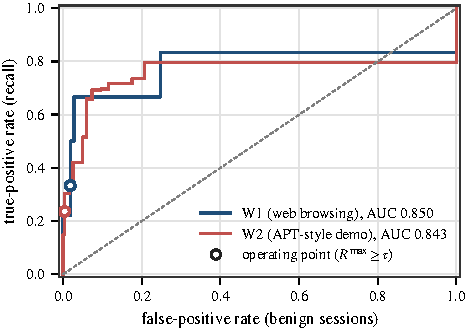
\includegraphics[width=0.82\columnwidth]{figures/roc.pdf}
\caption{ROC curves over the session peak risk for one representative seed
(seed~0, AUC 0.850 on W1 and 0.843 on W2; the 30-seed means are 0.884 and
0.851). The circles mark the operating point of the calibrated threshold.}
\label{fig:roc}
\end{figure}

On both datasets SICA kept the false-positive rate below 1\% on average, and
more than nine out of ten alerts were real hijacks. When SICA alerted, it did so
early, after a median of 1.4 (W1) and 2.5 (W2) attacker requests. Recall,
however, was limited: SICA found about a third of the hijacks on W1 and fewer
than a quarter on W2. The ROC curves in Fig.~\ref{fig:roc} show why. They
rise steeply at low false-positive rates and then flatten: one group of hijacks
receives a high peak risk, while many others receive the same low peak as a
benign one-way move, or no risk at all. SICA therefore favours a controlled false-alarm rate over
maximum attack coverage. IP pinning caught about 70\% of the hijacks but alarmed
on about 15\% of benign sessions. SICA is not better than pinning at finding
attacks, and several pinning rules reach a higher F$_1$ score. Its advantage is
a false-alarm rate that is an order of magnitude lower and chosen in advance,
together with an explanation for every alert. When hijacks are rare, this
matters more than raw coverage~\cite{axelsson2000baserate}. The budget can
also be relaxed: at 5\%, recall rose to 0.646 (W1) and 0.445 (W2) with a
false-positive rate of 4.4\% and 3.9\%.

\subsection{What SICA Detects and Misses}

Detection depends on what the attacker changes and on whether the victim keeps
browsing. Against an attacker on another network with their own browser (L0) in
concurrent mode, recall was 0.993 on W1 and 0.893 on W2. When the attacker
copied the User-Agent from another network (L1), V1 could not fire, but the
binding fork still caught 70\% (W1) and 72\% (W2) of the concurrent attacks. The
same attack as a silent takeover was almost never caught (recall 0.002 and
0.001), because it looks like a one-way move. An attacker with the victim's
exact IP address and User-Agent (L4) cannot be detected from these fields at all.
On the benign side, address changes within a /16 and browser updates never
caused an alert, while interface flapping across /16 networks alerted in about
58\% of such sessions and caused most false alarms.

\textbf{Limitations.} The attacks were injected into real traffic rather than captured from real
incidents, and the benign mobility rates are our assumptions. Both logs are
public samples; W2 is demonstration data with only three URLs, and the minute
field of both logs is degenerate, so we make no timing claims. Sessions were
rebuilt from (IP, User-Agent) rather than taken from real cookies.

% =====================================================================
\section{Conclusion}
% =====================================================================

In this project we built SICA, a lightweight detector that looks for
mid-session HTTP session hijacking using only the web server's access logs. SICA
describes each request by a client binding, scores agent changes, graded
network changes and the binding fork, and compares the session's peak risk with
a threshold calibrated on attack-free sessions. The project showed that
server-log-only detection is practical for one clear case: two clients using
the same session at the same time from different networks or different
browsers. On two public datasets, SICA kept the false-positive rate at 0.85\% and
0.56\% with precision above 0.9, while IP pinning alarmed on about 15\% of benign
sessions. Its recall was low (0.358 and 0.229). SICA cannot detect an attacker
who reproduces the victim's binding closely enough, and silent takeovers are
often indistinguishable from normal mobility. The next stage of the project can
investigate a larger and more diverse set of real-world logs and richer signals
while keeping the design lightweight and interpretable.

\bibliographystyle{IEEEtran}
\bibliography{report}

\end{document}
